\documentclass[12pt,a4paper]{report}

% === PACKAGES ===
\usepackage[utf8]{inputenc}
\usepackage[T1]{fontenc}
\usepackage{setspace}
\usepackage{geometry}
\usepackage{apacite}
\usepackage{graphicx}
\usepackage{titlesec}
\usepackage{fancyhdr}
\usepackage{newtxtext,newtxmath} % Times New Roman font
\usepackage[utf8]{inputenc}
\usepackage{gensymb}

%%\usepackage{textgreek}

% === PAGE SETTINGS ===
\geometry{margin=1in}
\onehalfspacing
\pagestyle{fancy}
\fancyhf{}
\fancyhead[L]{\leftmark} % Chapter title in header
\fancyfoot[C]{\thepage}
\renewcommand{\headrulewidth}{0.4pt}
\renewcommand{\footrulewidth}{0.4pt}

% === SECTION NUMBERING ===
\titleformat{\chapter}{\bfseries\large}{\thechapter.}{1em}{}

\renewcommand{\thesection}{\thechapter.\arabic{section}}
\titleformat{\section}{\bfseries\normalsize}{\thesection}{1em}{}

\renewcommand{\thesubsection}{\thesection.\arabic{subsection}}
\titleformat{\subsection}{\bfseries\normalsize}{\thesubsection}{1em}{}



% === TITLE PAGE ===
\begin{document}
	
	\begin{titlepage}
	\centering
	
	{\Large \textbf {\underline{A critical review of electrosynthesis of Metal Oxide Semiconductors}}\par}
	\vspace{0.5cm}
	
	{\it submitted to the\par}
	\vspace{0.4cm}
	
	{\large\textbf{INSTITUTE OF CHEMICAL TECHNOLOGY, MUMBAI}\par}
	\vspace{0.2cm}
	
	{\it for Partial fulfillment of the degree of\par}
	\vspace{0.2cm}
	
	{\large Bachelors of Chemical Engineering\par}
	{\large (Semester VII)\par}
	\vspace{0.5cm}
	
	{\large by\par}
	\vspace{0.3cm}
	
	{\Large Nidhi Kulkarni\par}
	{\large 22CHE142\par}
	
	\vspace{1cm}
	
	% ---- Insert Institute Logo ----
	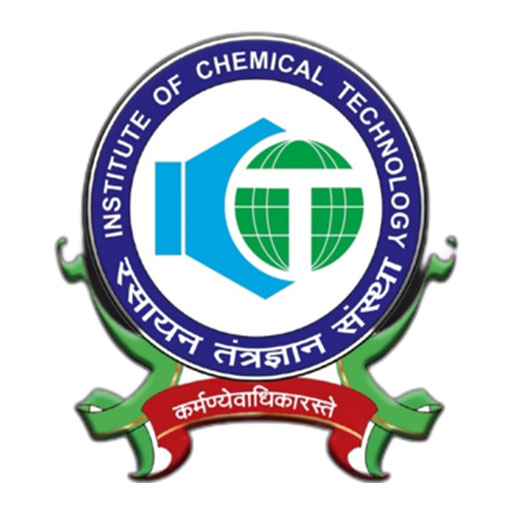
\includegraphics[width=0.3\textwidth]{figures/ictlogo.jpg}\par
	% Replace 'logo.png' with your actual file name in the same folder.
	
	\vspace{1cm}
	
	{\large Institute of Chemical Technology, Mumbai\par}
	\vspace{0.2cm}
	
	{\small (University Under Section 3 of UGC Act 1956;\par}
	{Elite Status and Centre of Excellence, Government of Maharashtra)\par}
	
	\vspace{1cm}
	
	
	
	{\large November 2025\par}
	
	\vfill
	\begin{flushright}
		\textbf{AVP} \\ % Replace ABC with supervisor's initials
	\end{flushright}
	\end{titlepage}

	
	% === INDEX ===
	\tableofcontents
	\newpage
	\listoffigures
	\addcontentsline{toc}{chapter}{List of Figures}
	\newpage
	
	

	
		% === ABSTRACT ===
	\chapter*{Abstract}
	\addcontentsline{toc}{chapter}{Abstract}
	In this seminar report, we discuss electrosynthesis of Metal oxide semiconductors. We focus on the recent advances in this field and applications of this method as stated in the literature. Electrosynthesis is a recent method for making metal oxide semiconductors that has been developing since the 1970s. Here we discuss the method in detail and talk about the uses and applications of electrosynthesis of metal oxide semiconductors as stated in literature. This study details the electrochemical fundamentals that define potentiostatic and galvanostatic modes of deposition. Additionally, this article provides an overview of the recent advancements made within the field of electrochemistry, including anionic-assisted electrodeposition, hydrogen doping, morphological templating, and advancements in improving interfacial chemistry and structural characterization. Furthermore, this review compiles the various ways in which electrosynthesized metal oxide semiconductors can be utilised within different technology areas, including electronic devices (metal oxide semiconductor field effect transistors (MOSFETs), cross-point memory), energy conversion and storage systems (photoelectrochemical water splitting, quantum dot-sensitized solar cells, supercapacitors, and batteries), environmental monitoring sensor systems (gas and biosensors), fuel cells, as well as emerging applications in catalysis and plasmonic. The benefits of electrosynthesis include: precise control of composition; scalable, low-temperature processing; tunable morphologies; and very little production of by-products – all of which make electrosynthesis an attractive and economical method for developing advanced functional materials. However, challenges still exist with respect to cathode corrosion and maximisation of process parameters. Recent developments in the understanding of electrochemical mechanisms and in-situ characterisations, in combination with the advent of machine learning-based process optimisation methods, represent an opportunity for the continued expansion of electrosynthetic opportunities for next-generation semiconductor technologies.
	
	% === CHAPTER 1 ===
	\chapter{Introduction}
	The semiconductor industry has been seeing a surge in demand due to the recent developments in the electronics and allied industries. Metal Oxide Semiconductors (here by, abbreviated as MOS) are of growing interest due to the range of morphology, conductivity and sensitivity. \cite{Haynes2015}. This allows MOS  to be used in fields of PEC applications, sensors, hydrogen production and even energy storage. \cite{Rajeshwar2004}.  Rare earth metal oxides are used in television, wind turbines, LED light bulbs, and cell phones. \cite{Patil2022} MOS are different from traditional metal oxides in the aspect that MOS are highly conductive due to their large bandgaps and localized electron states while metal oxides are either insulative or resistive. Due to the diverse applications, it is necessary to develop MOS using an inexpensive, facile and universally applicable method that provides flexibility in control and morphology of the MOS crystals. 

	
	\section{Methods to synthesize MOS}
	There are several methods to synthesize MOS such as Hydrothermal, Precipitation, Micro-Emulsion, Microwave assisted, Sol-gel, Vapour deposition and Electrosynthesis. Here we discuss the major methods used for making MOS devices.
	
	\subsection{Hydrothermal}
	Hydrothermal synthesis utilizes high temperatures and high pressures to produce MOS. The first hydrothermal synthesis ever made was by the German geologist Karl Emil von Schafhäutl in 1845, who succeeded in growing microscopic quartz crystals in a pressure cooker. Hydrothermal methods are the best to manufacture nanoparticles as reviewed by Medhi et. al \cite{Medhi2020} Despite its apparent advantages, such as the possibility of synthesizing crystalline phases that are unstable at their melting points and the chance to grow large, good-quality single crystals, the hydrothermal method has a number of disadvantages. Among the disadvantages are the following: rather expensive autoclaves and special equipment to resist extreme conditions, impossibility of observation of crystal growth when using steel vessels, which complicates the control of phase composition and makes the reaction process difficult to control and interpret since the pressure vessel is closed. (K. Byrappa, “A Handbook of hydrothermal Technology”, Noyes Publications, pp. 1-10, 2001)
	\begin{figure}[h!]
		\centering
		\fbox{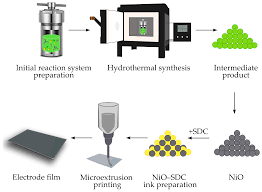
\includegraphics[width=12cm,height=10cm,keepaspectratio]{figures/fig1.png}}
		\caption{Setup for Hydrothermal Synthesis}
		\label{fig:hysteresis}
	\end{figure}
	
	\subsection{Sol-gel}
	Sol-gel is a critical process for preparing inorganic materials and is playing an important role in inorganic synthesis. In the process, organometallic compounds or organic complexes produce a sol at low temperatures, form a gel under certain conditions, and then undergo heat treatment. That is, the ultra-fine nano powder with a bigger specific surface and better dispersion may be obtained by preparing the homogeneous solution, the sol, the gelation process, the drying of the gel, and the heat treatment process of the xerogel. The procedure can be performed under mild conditions, and the resulting powder has a larger surface and strong dispersibility; however, the reaction time is longer and requires several days to finish, which is not able to meet the criteria of large-scale manufacturing. \cite{Patil2022}
	\begin{figure}[h!]
		\centering
		\fbox{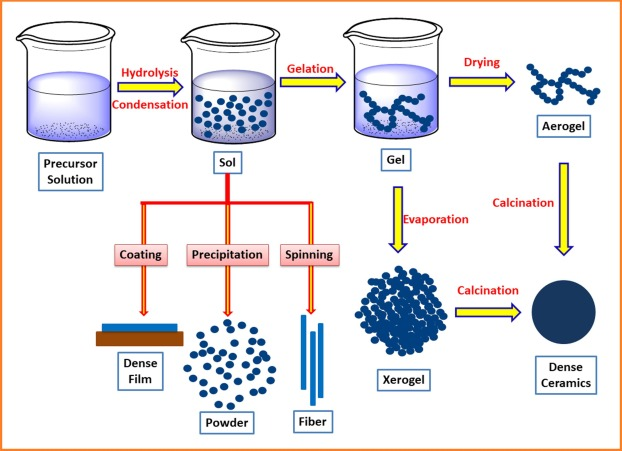
\includegraphics[width=12cm,height=10cm,keepaspectratio]{figures/fig2.jpg}}
		\caption{Sol-gel Synthesis}
		\label{fig:hysteresis}
	\end{figure}
	
	
	\subsection{Vapour Deposition}
	Chemical Vapor Deposition (CVD) is a type of vacuum deposition technique used for creating high-quality and high-performance solid and thin films. In conventional CVD processes, the semiconductor wafer or substrate is subjected to one or more volatile precursor species, which then react and/or decompose on the wafer’s surface, thereby creating the desired material. The process uses chemical reactions within a heated high-vacuum deposition system, which is usually carried out at temperatures above 900°C, and is used to produce thin-film layers and other advanced nanotechnology constructs through various types of chemical vapor deposition processes. The chemical precursors are continuously introduced into the chemical precursor deposition reactor, then transported toward the semiconductor material surface through various fluid transportation processes, and then the resultant deposited solid layer is formed while removing by-product species from the deposition reaction chamber. 
	The primary disadvantages of this method are high process temperatures, hazardous precursors and by-products, physical and logistical constraints, difficulty with multi component materials and high equipment and precursor costs. \cite{Swain2015}
	
	\begin{figure}[h!]
		\centering
		\fbox{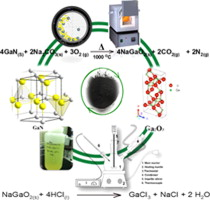
\includegraphics[width=12cm,height=10cm,keepaspectratio]{figures/fig3.jpg}}
		\caption{Vapour Deposition}
		\label{fig:hysteresis}
	\end{figure}
	
	\subsection{Electrodeposition(ED) or Electrosynthesis (ES)}
	Electrosynthesis is defined when the diffusing species being charged and the diffusion medium being porous or layered to have an induced diffusion by changing the current or the potential. Unlike the chemical synthesis technique, electrosynthesis uses electric currents to electrochemically reduce and oxidize chemical substances on electrodes, hence directly converting chemical precursors into solid products. There are novel electrosynthesis techniques which are easy and cheap alternatives to chemical synthesis techniques for preparing ceramic thin films, nano-particulate material, and metastable phases, which are difficult to synthesize by chemical synthesis techniques. The main benefit of electrochemical synthesis is the control exerted on the deposition process by controlling electrochemical reaction variables, which enables the synthesis of high-quality and high-purity material directly on the surface of substrates without generating any unwanted by-products. \cite{Therese2000}. It also allows us to produce MOS of varied morphologies (nanorods, films, crystals etc.) and can manufacture both p-type and n-type semiconductors. ED can be used to make semiconductors in either bulk or film form. \cite{Rajeshwar2006}
	The disadvantages of this method are the difficulty in characterization of the product, presence of X-ray impurities and the use of only conducting raw materials. However, since any conducting substrate can be used to make the MOS and the possibility of even combining more than one substrate makes this method far more superior than any of the other synthesis methods.
	\begin{figure}
		\centering
		\hbox{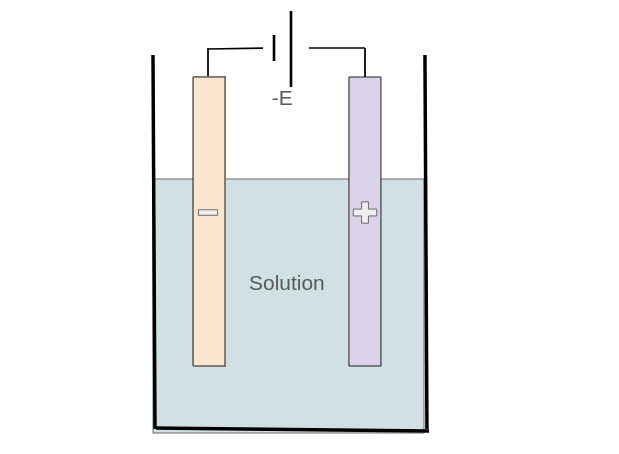
\includegraphics[width=12cm, height=10cm]{figures/fige.png}}
		\caption{Setup of electrosynthesis}
		\label{fig:hysteresis}
	\end{figure}
	
	
	% === CHAPTER 2 ===
	\chapter{Overview of Electrosynthesis}
	The versatility of this method makes it an important way to synthesize MOS as talked about in Garvonskii et. al. \cite{Garnovskii1999}. The methods for electrosynthesis can be classified based on the type of control and the main reaction used for electrosynthesis.
	\section{Types of Electrosynthesis based on control}
	The progression of the reaction is mainly influenced by two factors: \textbf{(i)} the deposition current and \textbf{(ii)}the cell potential. During the reaction, one can choose to control either one of these factors as a function of time. When the deposition current is controlled, it is called as \textbf{Galvanostatic synthesis} and when the cell potential is controlled it is called as \textbf{Potentiostatic synthesis}.
	
	\subsection{Potentiostatic electrosynthesis}

	Potentiostatic electrodeposition is a technique in which the potential of the working electrode is held constant relative to a reference electrode. 
	This ensures that the thermodynamic driving force for electron transfer remains 
	fixed, enabling precise selection of desired redox pathways and the suppression 
	of side reactions \cite{Isaev2020}. This type of synthesis is used when the making of the MOS is possible at any value between the initial potential $E_i$ and final potential $E_f$. It often uses a three electrode system.
	
	
	\subsubsection{Three-Electrode Configuration}
	The three electrode system as mentioned previously consists of Working electrode (WE),Reference electrode (RE) and Counter electrode(CE). This setup is described by \ref{fig:hysteresis}
	
	\begin{figure}[h!]
		\centering
		\fbox{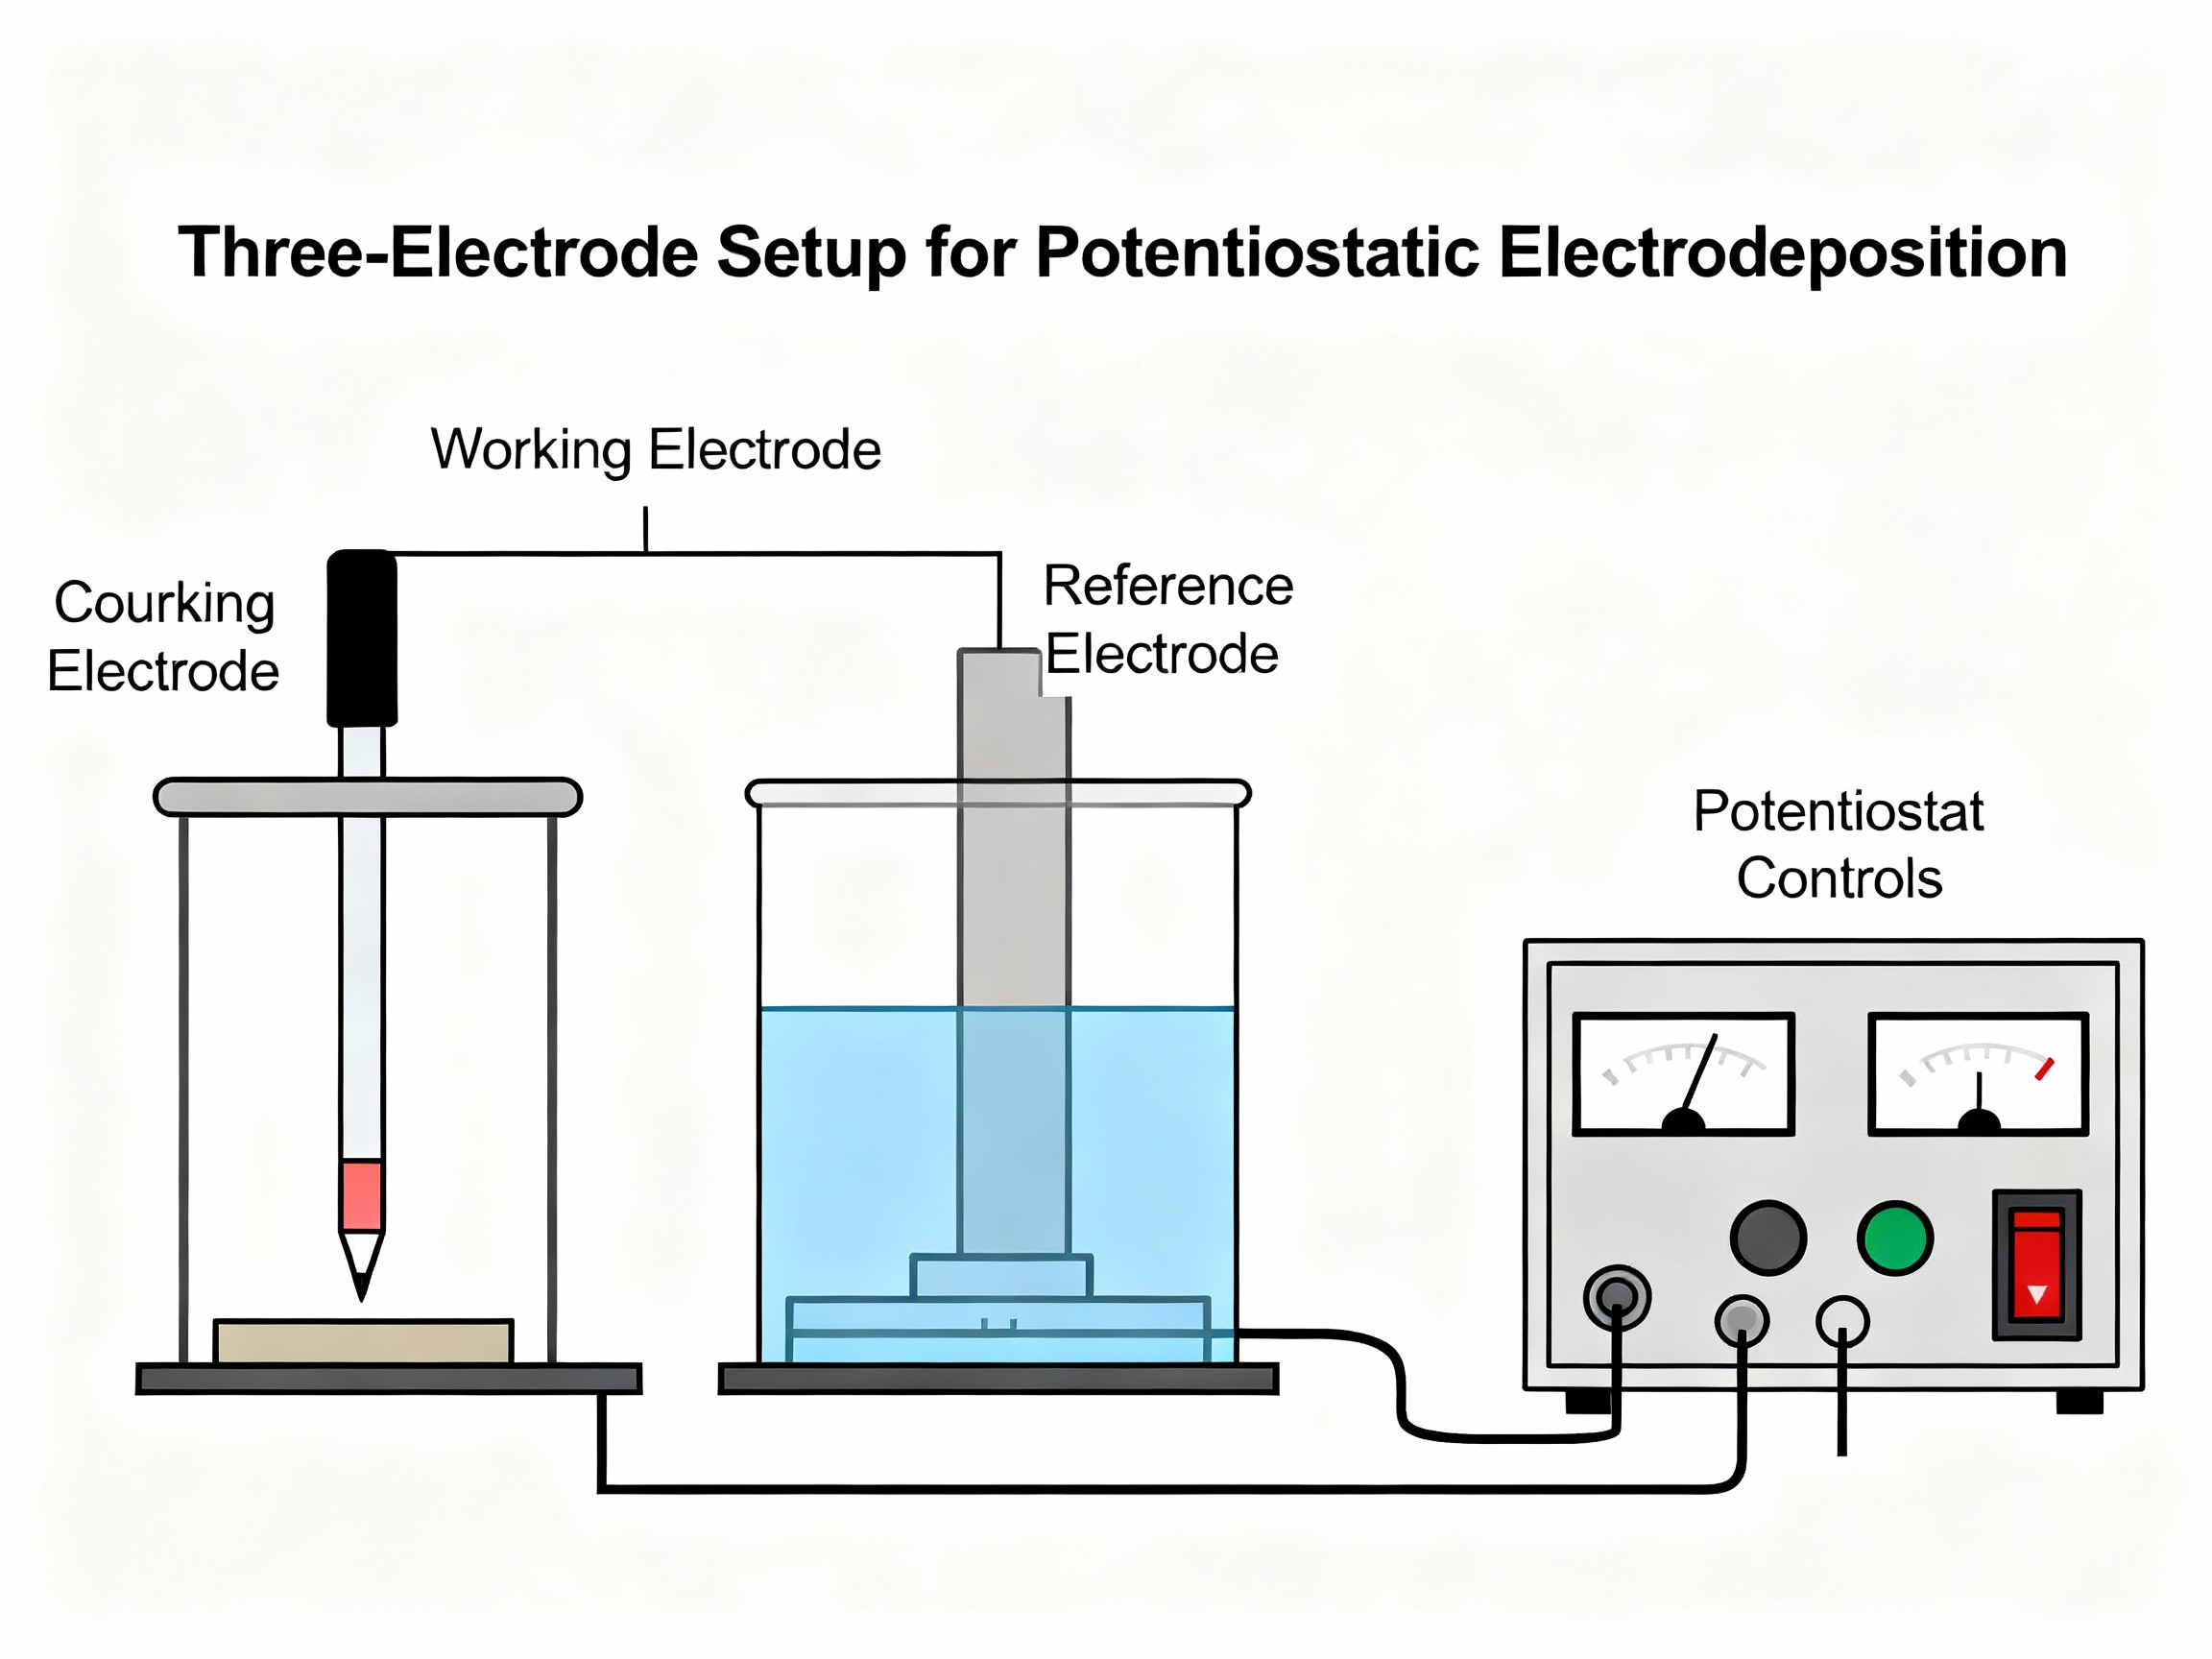
\includegraphics[width=12cm,height=10cm,keepaspectratio]{figures/figa.jpeg}}
		\caption{Three electrode setup used in potentiostatic synthesis}
		\label{fig:hysteresis}
	\end{figure}
	
	The potentiostat makes continuous adjustments to the current between WE and CE in order to hold the potential between RE and WE at the desired constant value. In this way, the system virtually eliminates all of the drop in potential due to resistance as seen in two-electrode systems, and more precisely enables manipulation of reaction thermodynamics.\cite{Harrar2013}.
	
	\subsubsection{Thermodynamic Control}
	
	The electrode potential determines the relative activity of oxidized and reduced
	species through the Nernst equation:
	
	\[
	E = E^\circ + \frac{RT}{nF}
	\ln \left( \frac{a_{\mathrm{ox}}}{a_{\mathrm{red}}} \right).
	\]
	
	Depending on whether the potential is positive or negative, the deposition can be of two types
	
	\textbf{1. Under-potential Deposition (UPD)}
	Occurs at potentials more positive than the bulk equilibrium potential. It
	produces monolayer or sub-monolayer films with strong surface-specific
	selectivity \cite{Isaev2020}.
	
	\textbf{2. Over-potential Deposition (OPD)}
	Occurs at potentials more negative than equilibrium. It produces
	three-dimensional growth and thick films.
	
	\subsubsection{Kinetics and Current-Time Behaviour}
	
	Upon imposing a potential step, the current transient typically contains two
	components:
	
	\begin{enumerate}
		\item \textbf{Double-layer charging}, decaying exponentially.
		\item \textbf{Faradaic current}, often diffusion-limited and described by the
		Cottrell equation:
		\[
		i(t) = \frac{n F A C_0 D^{1/2}}{\pi^{1/2} t^{1/2}}.
		\]
	\end{enumerate}
	
	Nucleation mechanisms—instantaneous or progressive—can be identified by
	comparing experimental transients to the Scharifker-Hills theoretical forms
	\cite{Yuan2021}.


	
	\subsubsection{Advantages and Limitations}
	
	Potentiostatic deposition enables:
	single-phase, thermodynamically selected products,high reproducibility for nanostructures, mechanistic studies through current-time transients,precise control over alloy composition.

	
	Limitations include:
	
	\begin{itemize}
		\item decreasing current with time due to reactant depletion
		\item slow growth rates for thick films
		\item sensitivity to reference electrode stability
		\item noise at very low currents.
	\end{itemize}
	
	
	Potentiostatic control provides superior thermodynamic precision and mechanistic
	clarity compared to galvanostatic deposition. It is therefore the method of
	choice for research on nanostructures, catalytic materials, and fundamental
	electrode kinetics, although its slower deposition rate can be a drawback in 
	industrial contexts. \cite{Xi2014}
	
	
	
	\subsection{Galvanostatic electrosynthesis}
	Galvanostatic electrodeposition is an electrochemical method in which the
	current density is held constant while the electrode potential evolves to 
	maintain the imposed current. Since the controlled parameter is current,
	the system adjusts its potential continuously to compensate for changes in
	reactant concentration, electrode surface conditions, and electrolyte resistance
	\cite{Schotten2020}. This makes galvanostatic deposition particularly attractive for large-scale and industrial electrodeposition where uniform current delivery
	and simplified instrumentation are required.
	
	\subsubsection{Electrochemical Basis}
	
	In a galvanostatic mode, the applied current density \( j \) is fixed:
	
	\[
	j = \frac{I}{A} = \text{constant},
	\]
	
	and the electrode potential \( E(t) \) becomes a time-dependent variable.
	The evolution of potential reflects changes in reaction kinetics, mass
	transport, and the formation of intermediates on the electrode surface. \cite{Jadhav2021}
	
	Faraday’s law relates the mass of deposited material to the applied current:
	
	\[
	m = \frac{I t M}{n F},
	\]
	
	where \( M \) is the molar mass of the metal, \( n \) is the number of
	electrons transferred, and \( F \) is the Faraday constant.
	
	\subsubsection{Potential Drift and Its Consequences} %%write again from here
	
	A key characteristic of galvanostatic synthesis is the drift of the cell
	potential. As electroactive species are consumed near the electrode, 
	their activity decreases, often requiring more negative potentials 
	to maintain the imposed current. This may lead to activation of secondary reactions,incorporation of impurities and formation of multiphase deposits.
	\cite{Zhu2024}
	
Figure~\ref{fig:fig4} illustrates the characteristic increase in
potential during a galvanostatic deposition experiment \cite{Norikawa2020}.

\begin{figure}[h!]
	\centering
	\fbox{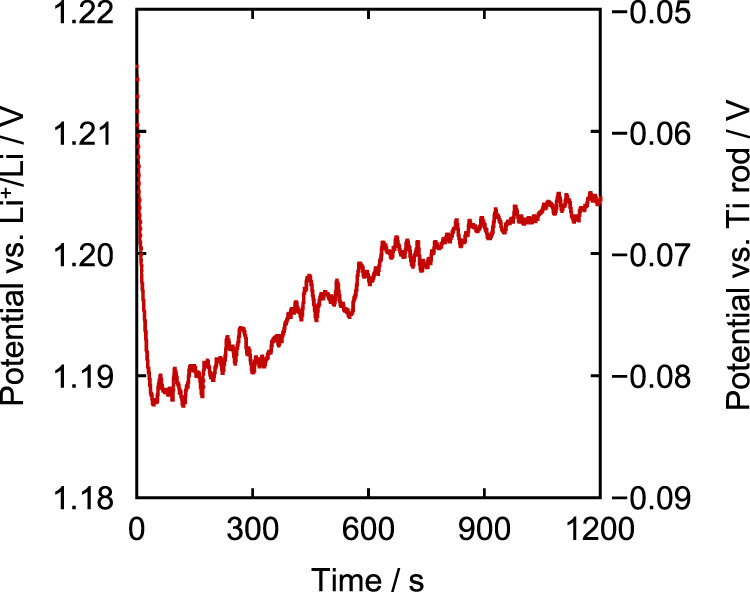
\includegraphics[width=12cm,keepaspectratio]{figures/fig4.jpg}}
	\caption{Potential drift in galvanostatic synthesis (ref. Norikawa et al.)}
	\label{fig:fig4}
\end{figure}

	
	\subsubsection{Advantages and Limitations}
	
	Galvanostatic control provides uniform current distribution across large surfaces,simplicity of hardware and 
	compatibility with industrial processes.
	However, it suffers from poor thermodynamic selectivity,potential drift leading to multiple phases, sensitivity to electrode geometry and mass transport limits. 	Galvanostatic electrodeposition is robust and industrially versatile, but the
	lack of thermodynamic control over electrode potential can lead to variability
	in composition and morphology. It is best applied when deposition rate and 
	uniformity are more critical than phase purity or mechanistic insight. \cite{LopezSauri2015}
	
	Thus, while galvanostatic control is widely used in practical plating and 
	coating processes, it is less suited for mechanical investigations or for
	precised nanoscale synthesis.
	


	
	
	\section{Types of Electrosynthesis based on governing reaction}
	
	\subsection{Anodic oxidation}
	When the oxidation occurs at the anode during electrosynthesis,such synthesis is called as anodic oxidation. \cite{Li2024}. This method is widely used to synthesise MOS films and nano particles directly on the metal substrate. It offers a precise control over thickness, morphology, and semiconducting properties. Often Ni or W based metal oxide semiconductors are processed using this method \cite{Therese2000}. 
	This method allows to efficiently separate charge upon integration of the systems to photoanodes has been attributed to the placement of the conduction bands at appropriate energy levels for the oxidation of water and the degradation of contaminants through photo-electro-chemical(PEC) reactions, and their respective band gaps and the potentials of their corresponding flat bands. \cite{Zych2020} 
	Despite the advantages in cost and ease of variability in morphology of the MOS, this method is dependent on an underlying metal (i.e. metallic anodes limit substrate options). There is a chance of possible inhomogeneity or breakdown at elevated operating voltages or during post-annealing that can limit the advantages offered by this process. A tight balance must be maintained between growth and dissolution in fluoride-based systems due to the risk of excessive chemical etching resulting in delamination or structural collapse of nanotubes/pores limiting the scope of available operating parameters for reproducible semiconductor architectures are just some of the limitations associated with the materials. \cite{Chiang2025}
	\subsection{Cathodic reduction}
	Cathodic reduction is a half-reaction in which an entity gains electrons at the cathode (where reduction occurs) and serves as a foundation for a plethora of different types of electrosynthesis/electrocatalysis in both organic and inorganic chemistries. \cite{PLETCHER201597} Modern-day electrosynthesis uses cathodic reduction to activate strong bonds, provide the reactive intermediates required for reactions between small molecules (such as $CO_2$) under controlled, environmentally friend's conditions, generate reactive intermediates, etc. To enhance the selectivity of $CO_2RR$ (where $CO_2RR$ is the reaction for producing hydrocarbons from $CO_2$). \cite{Lei2009}many studies using metal-oxide based catalysts (Cu, Zn, mixed oxides) have been conducted focusing on two major components associated with the $CO_2RR$ reaction- 1) what oxidation state(s) the surface of the catalyst is/are in at the point of being an electrode (the oxide surface) and 2) what pH exists at the interface region (cathode-electrolyte interface). Op-ando spectroscopy studies using Cu-based electrodes show that copper (Cu) surfaces develop dynamically evolving Cu(I)-O species and Cu-Zn metals (the heterometal ensemble) with cathodic current and that these developing species and ensembles govern the pathways of both hydrogen evolution and $CO_2$ hydrogenation that answer why interfacial chemistry controls cathodic reduction selectivity.
	Cathodic reduction faces a significant challenge due to the corrosion of the cathode materials (electrodes) experienced by metal cathodes when exposed to either negative electrical potential or a strong concentration of aggressive cationic species in solution.\cite{Wirtanen2021}  The authors of these investigations have presented four possible solutions to mitigate this type of corrosion: 
	\begin{enumerate} 
		\item {Use an alloy that contains one or more metals as opposed to using a soft, pure, heavy metal} 
		\item {Add protective cationic compounds (i.e. specific alkali and/or ammonium salts)}
		\item {Adjust pH levels to provide a more favourable reaction environment}
		\item {Optimise the current density used in the electroreduction} 
	\end{enumerate}	
	These will enable the user to have a wider operating range for electroreduction, while decreasing the rate at which hydrogen gas is produced. The benefits of the above-described measures include, first, the increased durability of electrodes and, second, an increase in Faradaic efficiency and selectivity in cathodic reductions.
	
	\subsection{Electro-generation of base}
	Electrogeneration of base (EGB) is an electrochemical method whereby harshly basic materials are produced in situ at an electrode surface, typically at the cathode by using a reductive process rather than using the addition of stoichiometric quantities of chemical bases. The EGB method has gained significant use in both organic synthesis and the development of material chemistries because it allows for the production of deprotonated materials and produced precipitates through EGB processes in a much more environmentally friendly manner with more controllable, reproducible results compared to traditional methods. There have been numerous applications in the field of EGB regarding the cathodic electrosynthesis of vanadium oxide ($VO_x$) ceramic thin-films \cite{cite1}. Water or nitrate can be reduced electrochemically at the cathode, generating basic hydroxide that drives the subsequent precipitation and oxidation-dehydration of the carbonaceous species to produce vanadium oxide materials. As a result of this unique method of electrochemical oxides synthesis, large porous, high surface area vanadium axle materials have been manufactured that can be used as supercapacitor electrodes. These examples demonstrate how electrogenerated bases may serve not only as the reagent but also as the mechanism for delivering reagents in controlled localised and temporal locations for the synthesis of oxide and hydroxide materials without requiring the addition of alkaline reagents \cite{cite2}.
	
	The primary benefits of using Electrogenerated bases (EGBs) are numerous: strong bases (highly basic [alkaline]) can be generated on demand without having to add salt; EGBs generate high amounts of basicity very locally under relatively mild conditions at the bulk scale; it is easy to adjust the basicity of EGBs via adjusting potential, current density and electrolyte; therefore EGBs have "cleaner" post-reaction workups, produce much less salt waste, and are generally less harmful to sensitive functional groups than conventional base additions, making EGBs an attractive and environmentally friendly alternative.
	
	There are some drawbacks to using EGBs. Side reactions do occur that are a consequence of other electrochemical processes; these include competitive hydrogen evolution occurring at very negative potentials, electrode passivation and over-reduction of substrates present during EGB generation. \cite{cite3} For these reasons, it is necessary to carefully select appropriate electrode materials, solvents, cell configurations (divided versus undivided) and sometimes utilize "ex-cell" methods to exploit the potential of EGBs to their fullest and achieve consistent, high-quality results.
	
	
	\section{Advantages of electrosynthesis}
	The advantages offered by electrosynthesis for making MOS devices are as follows -
	\begin{enumerate}
		\item {Electrodeposition techniques enable the simultaneous formation of ternary oxide composites that exhibit enhanced capacitance and cycle stability} \cite{Abebe2022}.
		
		\item {Near the electrode, the electrochemical synthesis occurs at the electric double layer that possesses a very high potential gradient of 105 V cm-1. The reactions, often result in products which cannot be produced via chemical synthesis.}
		
		\item {The product is applied as a coating/thin film onto the electrode surface, and a solid-liquid interface will permit the conformal growth of such coatings/thin films on even the most irregularly shaped substrate when a counter electrode is used to ensure equal polarisation.} \cite{Therese2000}
		
		\item{The low-temperature method of electrochemical synthesis is limited by the boiling point of the electrolyte. 
		Melted salt electrolytes can be utilized to augment this.} 
		
		\item{An electrochemical synthesis occurs by using an oxidation or reduction reaction, and the power of oxidation or reduction can be continually and appropriately adjusted, by changing the potential applied to the cell—something impossible to accomplish with chemical synthesis.}
		
	\end{enumerate}
	
	
	% === CHAPTER 3 ===
	\chapter{Recent advances in Electrosynthesis of Metal Oxide Semiconductors}
	Electrosynthesis of metal oxide semiconductors (MOS) is a groundbreaking method for developing materials, allowing for control of morphology, composition and electronic properties through electrochemical deposition processes. In contrast to traditional synthesis methods such as chemical vapor deposition (CVD) or atomic layer deposition (ALD), electrosynthesis occurs at room temperature and under ambient pressure, allowing for the formation of metastable structures, and providing a route to scalable, functional materials. The controlling parameters for electrosynthesis are \textbf{pH, ligand in the solution, annealing temperature, agitation} and \textbf{the current density}. In this section, we will discuss recent developments in the electrosynthesis of metal oxides, including new synthesis methods, structural advances, and new applications in technology. 
	
	\section{Fundamental Principles and Methodologies}
	 
	\subsection{Core Electrochemical Principles}
	The electrochemical synthesis of metal oxides and hydroxides functions on a number of foundational principles that distinguish it from classic chemical synthesis methods \cite{Therese2000}. In the context of classifying, this method functions on a notion of "chimie douce", or soft chemistry, which promotes preservation of thermodynamically unstable phases and benign synthesis of metastable phases, via mild reaction conditions that may not be achieved by traditional high-temperature methods. Importantly, pH is a overwhelimgly influential control parameter in the deposition process that determines precipitation rates, phase selectivity, and final oxide composition.
	
	\subsection{Reduction of Processing Temperatures}
	Recent literature has demonstrated that electrochemical synthesis evolved from optimized electrochemical protocols has been able to radically reduce processing temperatures. For example, the templated electrosynthesis of zinc oxide nanorods in porous polycarbonate membranes \cite{Lai2006} has been able to reduce resultant crystallization temperatures relative to conventional processing temperatures. This significant reduction in temperature helps reduce energy consumption, but also enables integration with temperature-sensitive substrates and the scalability of manufacturing processes.  
	Similarly, solution-processed metal oxide semiconductors synthesized via facile redox reactions \cite{Chen2015}. Chen et al. reported temperature reduction in substrate annealing temperatures depending on the oxide composition. This provenance and temperature reduction is an important step forward in achieving energy-efficient manufacturing methods while reducing thermal shock to the substrate material.
	
	
	\subsection{Ligand Selection and Composition Control}
	The synthesis of indium-gallium-zinc oxide (IGZO) semiconductors via solution processing highlights the significant role ligands play in electrochemical synthesis methods established by Chen et al. The careful choice of organic ligands allows for a high degree of control over precursor reactivity and reproducibly produces high-purity metal oxide phases with diminished impurity incorporation, an issue that has long affected solution-processed oxides.
	
	
	\section{Advanced Synthesis Techniques and Innovations}
	
	\subsection{Anion-Assisted Electrodeposition}
	A significant methodological improvement uses anion insertion during cathodic deposition to facilitate the electrodeposition of durable metal hydroxide and oxide electrodes for oxygen evolution reactions\cite{Yan2018}. This has been described in \ref{fig:hysteresis}The method has two major benefits: first, it significantly decreases inter-facial resistance between the deposited oxide and underlying substrate, and second, it permits high mass loadings of deposits which can be linear equation $m = at + c$, where m is mass in milligrams and t is time in seconds. 
	\begin{figure}[h!]
		\centering
		\fbox{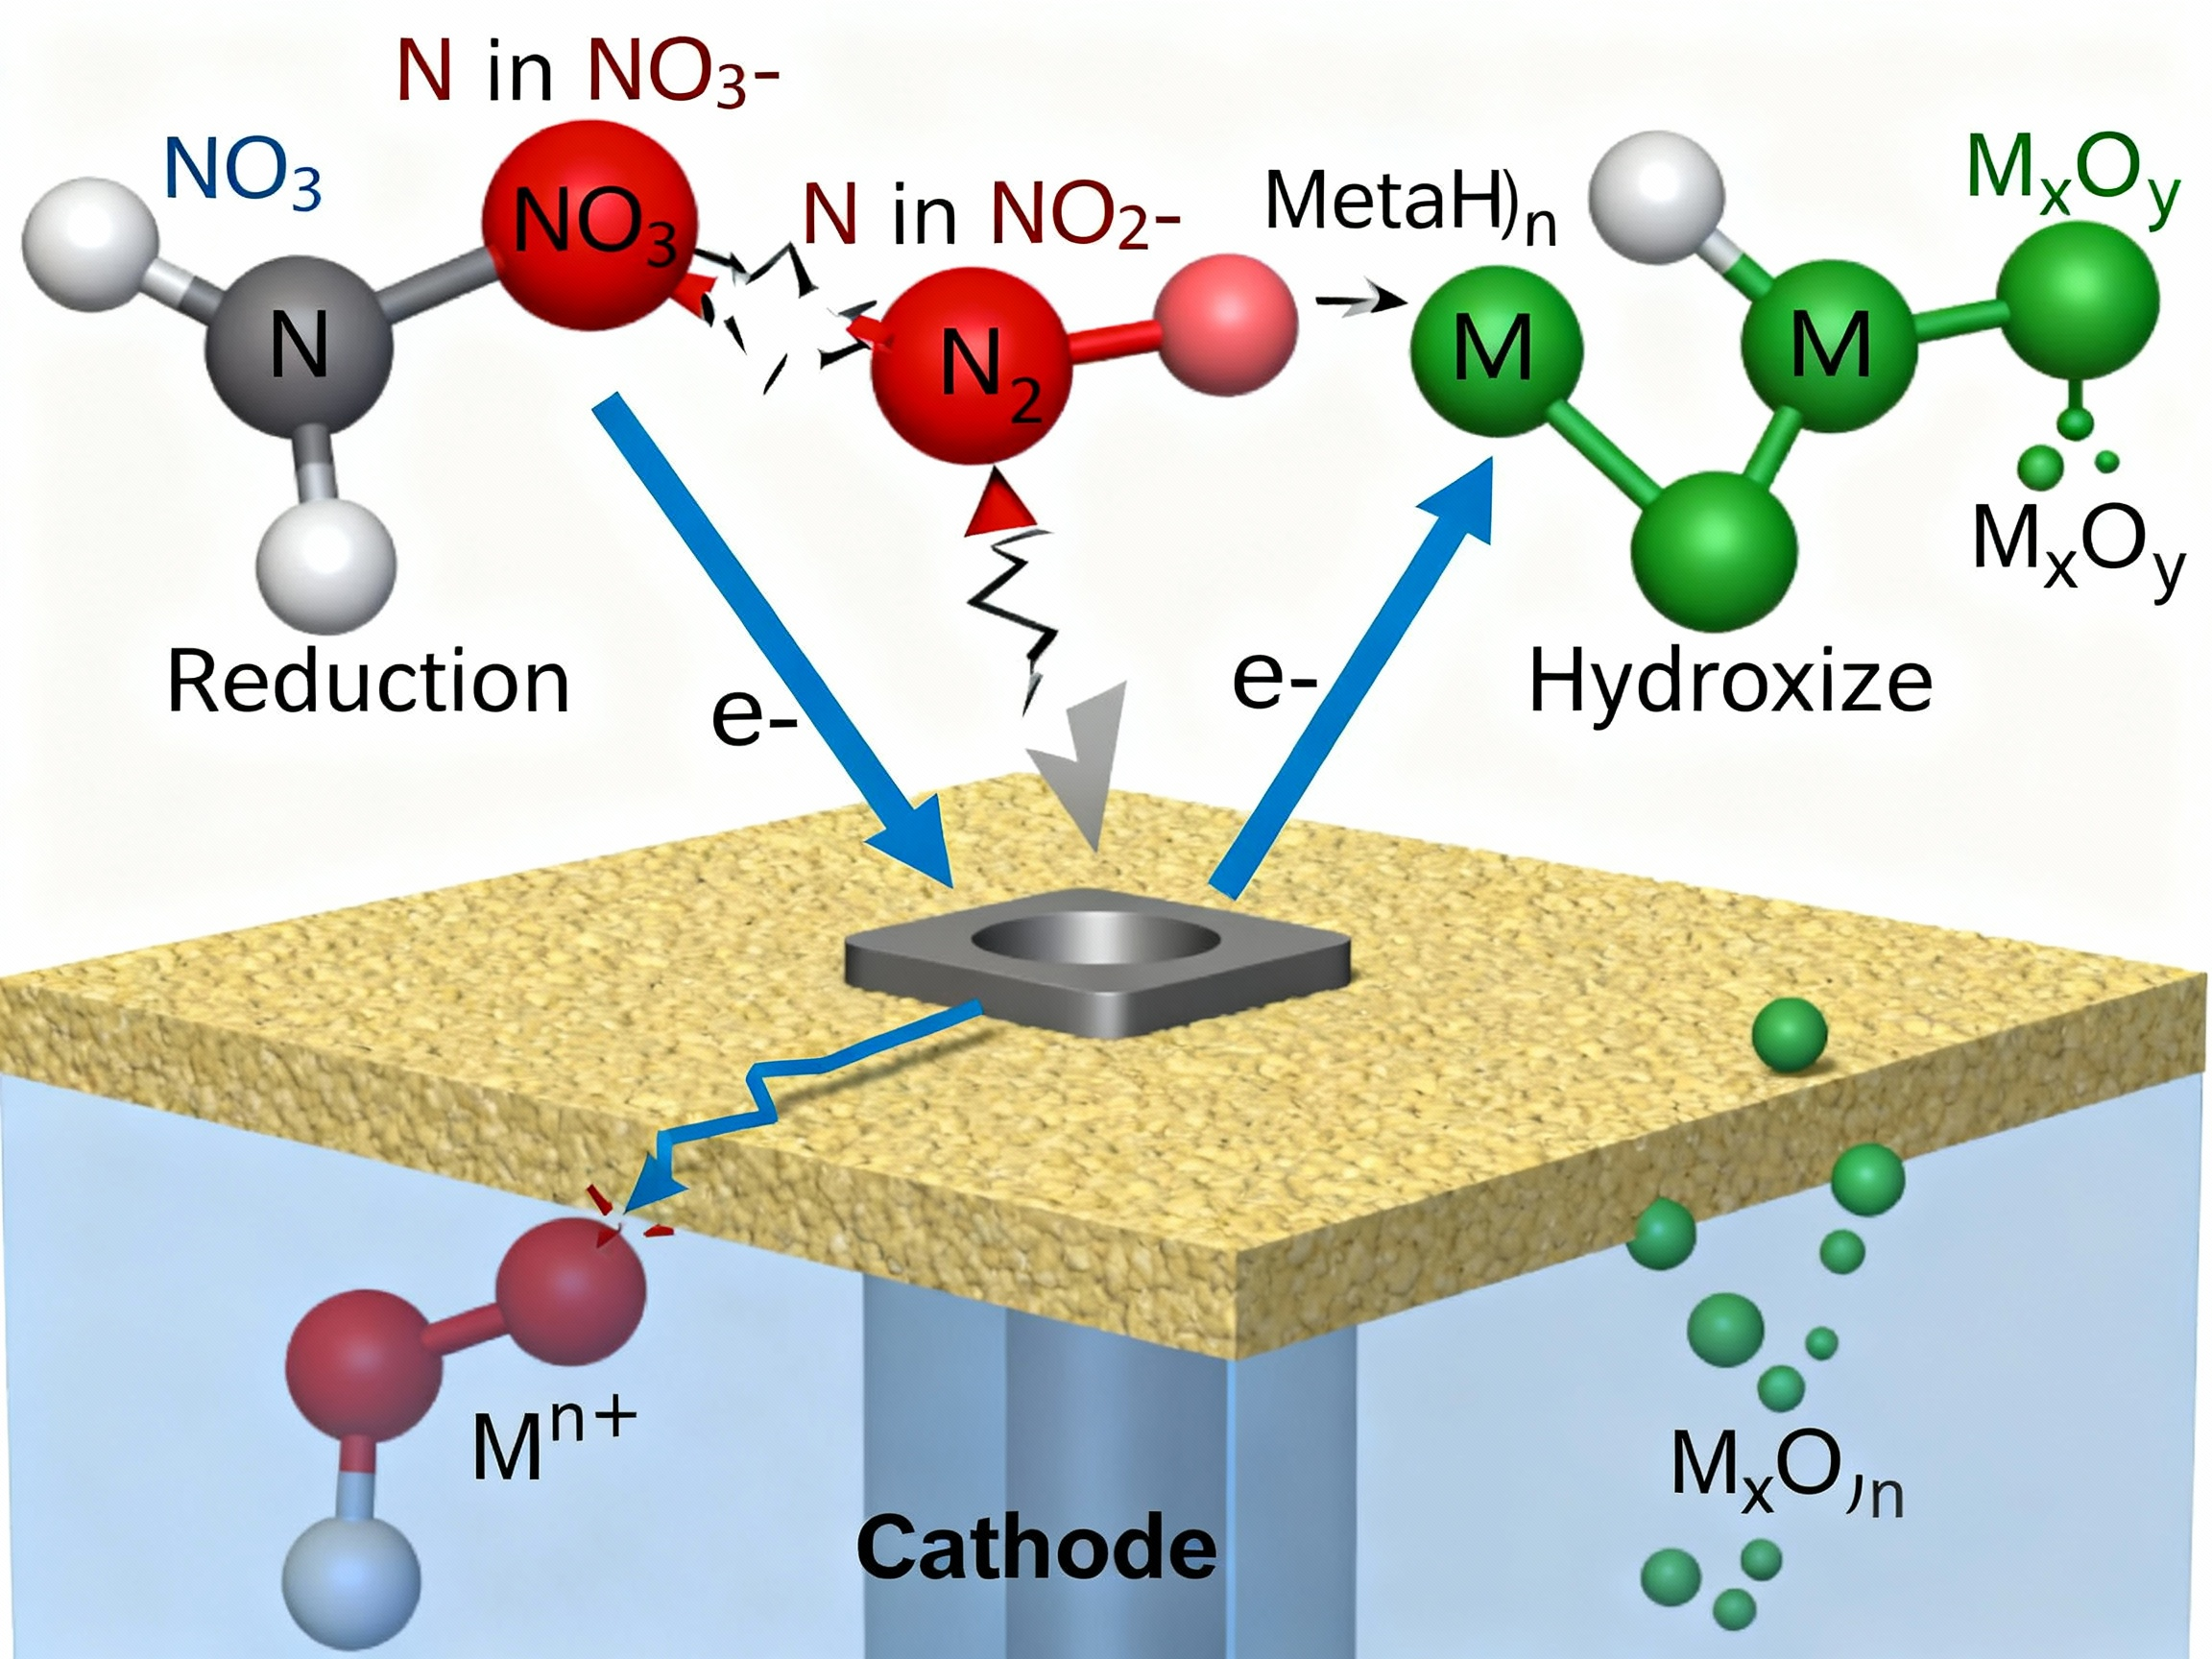
\includegraphics[width=12cm,height=10cm,keepaspectratio]{figures/figb.jpeg}}
		\caption{Mechanism of anion assisted electrodeposition}
		\label{fig:hysteresis}
	\end{figure}
	The methodology works by varying pH at controlled levels and adjusting conditions for anion intercalation, permitting the generation of complex heterostructures such as nickel-cerium systems with cerium oxide nanoparticles embedded within amorphous nickel oxyhydroxide (NiOOH) matrices.
	
	\subsection{Hydrogen-Doped Metal Oxide Semiconductors}
	Recent innovations in hydrogen doping have enriched the functional capacity of metal oxide semiconductors through Localized Suraface Plasmon Resonances (LSPR) \cite{Cheng2016}. Surface plasmon resonance (SPR) occurs when electrons in a thin metal film are excited by light directed at the film with a specific angle of incidence, and then propagate parallel to the film.Researchers have accomplished decreased hydrogen doping temperatures using palladium-based support materials down to room temperatures instead of the conventional temperatures of 400-550 \degree C. The support materials are Palladium and Silicon dioxide. This method also allows us to vary the range of the wavelength in which LSPR is observed by varying the temperatures.
	\begin{figure}
		\centering
		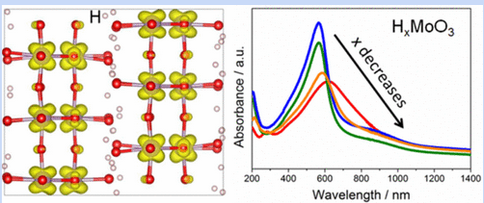
\includegraphics[width=12cm, height=10cm, keepaspectratio]{figures/fig6}
		\caption{LSPR phenomena observed in doped MOS. Source Cheng et.al}
		\label{fig:hysteresis}
	\end{figure}
	
	Exhibiting the hydrogen doping to the commercially available molybdenum trioxide ($MoO_3$) and tungsten trioxide ($WO_3$) provides systematically controllable optical absorption characteristics. Such characteristic can be utilized for optoelectronic and plasmonic possibilities.
	
	\subsection{Morphological Control Through Templating}
	Electrodeposition methods provide superior control over oxide semiconductor nanostructure morphology (i.e., thickness, shape, and electrical properties) because of what ED enables with regards to regulating solution-grown processes. This can be demonstrated in a simple approach using only an oven bath, spin coater, and potentiostat, supporting the standpoint that consistent, near-symmetrical, and highly ordered nanostructures can be created utilizing minimal equipment. Template-assisted methodologies also add geometry and further constrain electrochemical growth to geometric boundaries, allowing for the systematic production of uniformly sized nanorods, nanowires, and nanofilms within physically reproducible dimensions.
	
	This large degree of control over morphology becomes invaluable in applications that rely on modified surface area, charge-transport pathways, or optical properties, since these aspects of structural properties will influence conductivity, charge-carrier mobility, and overall photochemical performance. \cite{Lai2006}
	
	\subsection{Spatially Directed Electrosynthesis}
	Emerging methods utilize optical stimulation for spatially regulating the growth trajectories of semiconductor particles during electrosynthesis \cite{Rajeshwar2004}. Light directed electrodeposition allows for localized nucleation and growth at designated locations, which supports the formation of complex hierarchical architectures with detailed geometric order. This approach merges electrochemical synthesis with photonic control to yield new pathways toward programmable material synthesis.
	\begin{figure}[h!]
		\centering
		\fbox{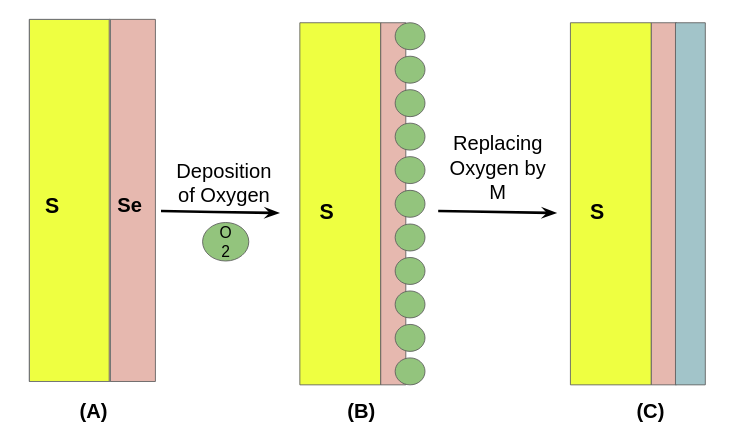
\includegraphics[width=12cm,height=10cm,keepaspectratio]{figures/figc.png}}
		\caption[The mechanism of deposition of Se on a template substrate S.]{In (A) the Se is in its natural 0 oxidation state. After cathodic deposition of Oxygen (B), the Se becomes $Se^{+2}$. Then the Metal ions $M^{+2}$ react with the SeO layer, displacing Oxygen and forming a MSe coating layer.}
		\label{fig:hysteresis}
	\end{figure}
	
	
	\subsection{Catalytic Metal Assisted Crystallization}
	Utilizes the example of aluminum serving as a catalyst to facilitate crystallization of metal oxide films made using solution processes at 400 $\degree$ C and 2mm thicknesses as optimal synthesis conditions, the crystallization of metal oxide films can be improved and varied to our preference if electrochemical synthesis is used. This type of metal-assisted crystallization is usually a cathodic reduction. We can change the crystal properties by changing the metal substrate species. The annealing temperature and the thickness can also be varied to our choice. \cite{Shin2020}
	
	
	
	
	\section{Enhancing the Inter-facial properties}
	
	\subsection{Interfacial Chemistry Optimization}
	Recent developments in tunable interfacial chemistry for controlling the electrosynthesis of metal oxide semiconductors \cite{Rajeshwar2023}, have highlighted challenges associated with corrosion-induced loss in conductivity for materials synthesized electrochemically. Careful modification of the interfacial chemistry, such as pH buffering capacity, surface charge characteristics, and electrolyte composition, can minimize the corrosive reaction while maintaining suitable electronic properties.

	
	\section{Structural Characterization and Predictive Modelling}
	After the manufacturing of the MOS, it is important to study the various electrical and chemical properties to predict and simulate the real life application of these devices. Computational techniques now make it possible to accurately predict electronic properties of electrosynthesized metal oxide semiconductors ahead of preparation \cite{Chanana2023}. Using fundamental relationships from Einstein relations and mass transport theory, researchers can indicate potential performance limits and electronic defects of specific oxide systems. The Einstein equation is as follows 
	$$\frac{dE}{E} = \frac{dM}{M} $$
	This predictive ability accelerates development cycles for materials by being able to identify new oxide compositions and potential performance limits which would eventually require effortful design interface. For example Chanana et.al study the $Ga_2O3$ MOS where it was found that the bulk electron mobility is low. 
	
	\section{Specific Oxide Systems and Their Synthesis}
	Synthesis of specific oxide systems can be done by varying the control parameters. For example, in the synthesis of Zinc Oxide nanorods by Lai et. al, a potentiostatic control was exerted over a solution containing Hydrogen peroxide and a salt of Zinc. The obtained nanorods were then studied by XRD methods.  \cite{Lai2006} It was also seen that the not all of the reduced hydrogen peroxide enable formation of Zinc Oxide hence the length of the nanorods was not directly proportional to the current passed. This has been demonstrated in the below figure.
	\begin{figure}[h!]
		\centering
		\fbox{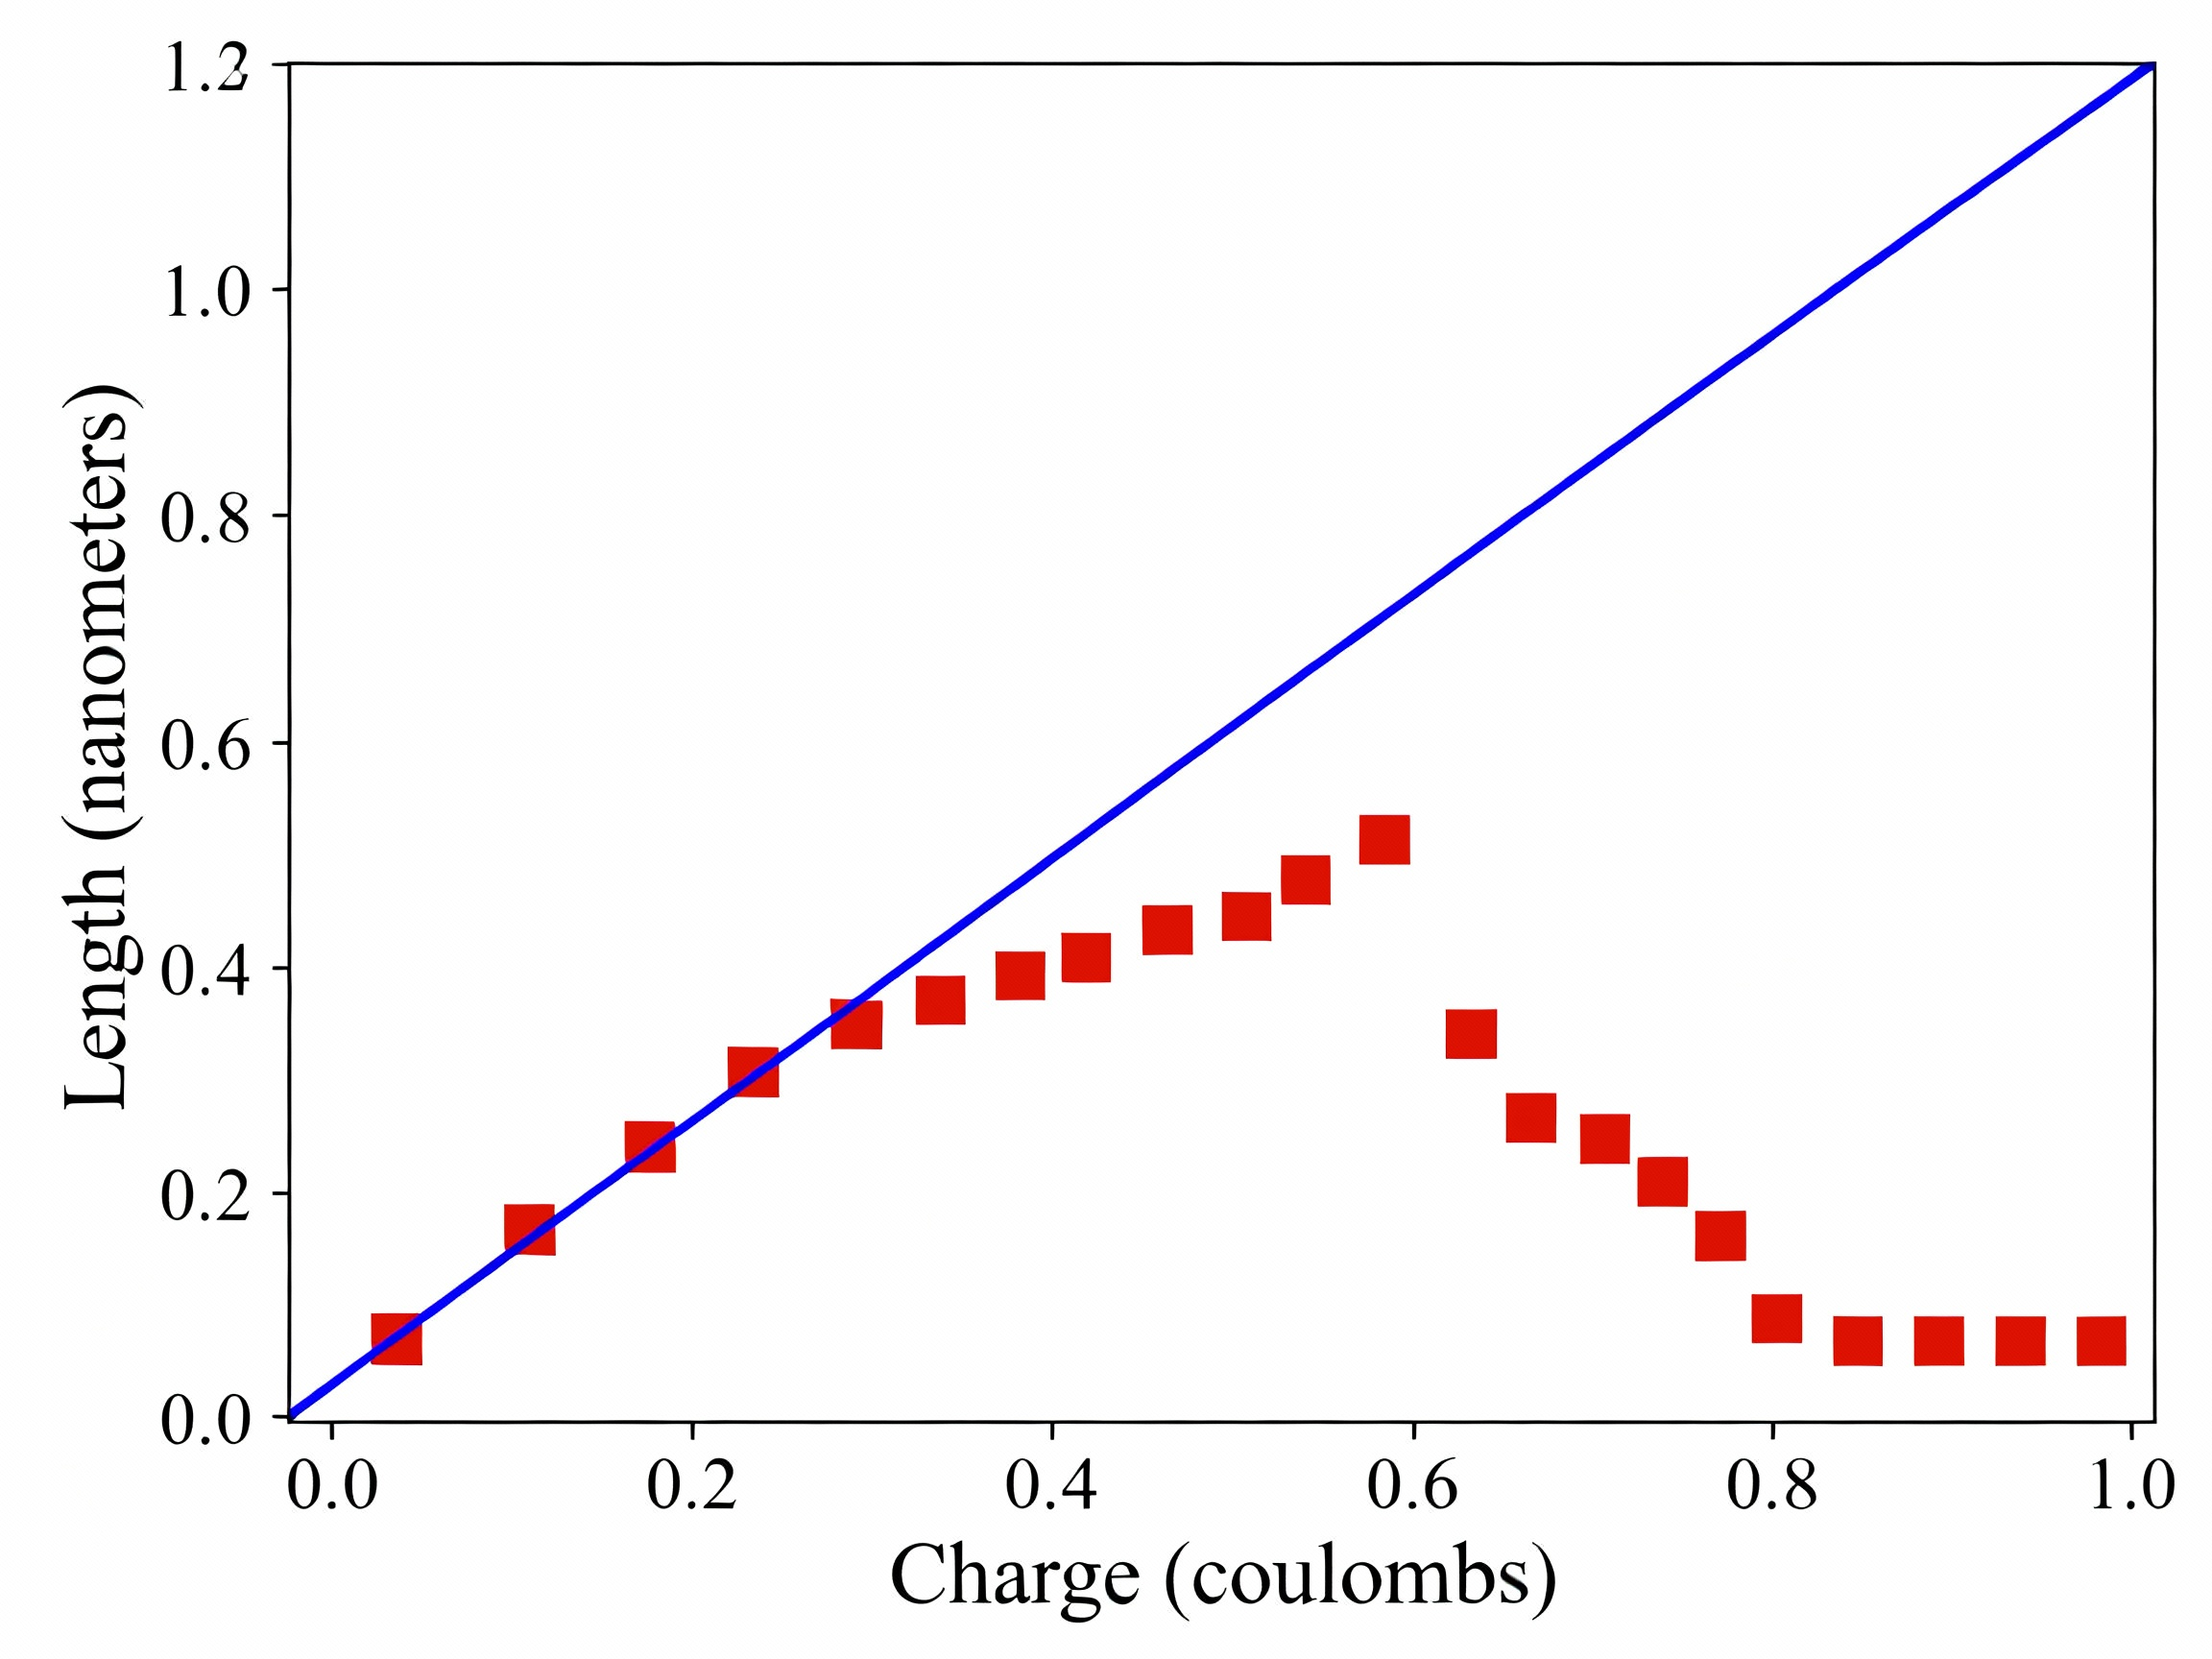
\includegraphics[width=12cm,height=10cm,keepaspectratio]{figures/figi.jpeg}}
		\caption{Plot of the length of nanorods in nm vs the charge passed}
		\label{fig:hysteresis}
	\end{figure}
	Similarly a study was conducted to synthize Curpous Oxide nanorods with a specific band gap of 2.2 eV. \cite{Haynes2015} Here again potentiostatic synthesis was used in a lactate stabilized Copper Sulphate solution. The morphology was controlled by the pH of the solution where a pH greater than 9 gave rise to formation of cubic crystals instead of nanorods. 
	The synthesis of a $AgO$ MOS device by Ida et. al \cite{Ida2008} is also another example of a one step synthesis of these devices by electrodeposition. The superior control that can be obtained by this technique results in being able to control the band gap of the MOS device.
	
	
	\section{Synthesis Challenges and Future Directions}
	Despite significant progress, there are still several unresolved technical challenges in metal oxide semiconductor electrosynthesis since it is a relatively newer method. The fundamental limitation of traditional metal oxide semiconductors in PEC applications has remained largely unchanged-namely, their high optical bandgaps greatly limit light absorption to ultraviolet \cite{Medhi2020}. This restriction remains a critical problem toward effective solar energy conversion. For the future, we will need to investigate bandgap engineering, including controlled doping, heterojunctions, and composite materials, if the light absorption strongly into the visible region is relatively easy to achieve. the research has also been carried out on relatively common and on similar metal ligands. Since this method of synthesis is universally applicable, more exploration should be done to expand the horizon of uses of this method.
	
	The advances in electrosynthesis of metal oxide semiconductors has led to the realization that electrochemical deposition is a broad and unique materials engineering platform for synthesis of metal oxide semiconductors at moderate synthesis conditions, while providing fine control over materials composition, structure, and properties. As improved electrochemical-based synthesis methods are applied in concert with theoretical modelling and device assembly methods, the scope of available oxide architectures expands along with discovering new functional properties. Ongoing developments toward spatially controllable synthesis approaches, interfacial engineering, and tuning band structure will further enable electrosynthesized semiconductors to increasingly accomplish demanding technological applications across diverse renewable energy conversion, advanced sensing, and memory devices.
	
	
	
	
	% === CHAPTER 4 ===
	\chapter{Applications and Uses}
	As discussed in the previous sections of this review, electrosynthesis has emerged as an important way to produce MOS and related devices. The electrosynthesis of metal oxide semiconductors (MOS) has developed into an exciting new field in both materials science and semiconductor engineering with the ability to finely control composition, morphology and interfacial properties. this routes allows the making MOS devices at milder conditions which is of great advantage industrially. In this section, we discuss the uses of this method as stated in literature. 
	
	\section{Applications in making electronic devices}
	\subsection{Metal-Oxide-Semiconductor Field-Effect Transistors (MOSFETs)}
	
	The fundamental application of these metal oxide semiconductors is the fabrication of metal-oxide-semiconductor field-effect transistors (abbreviated as \textbf{MOSFET}), which makes the cornerstone of modern integrated circuit technology \cite{Rajeshwar2023}. The ability to precisely tune interfacial chemistry can be achieved only by electrochemical synthesis since this methodology enables a controlled deposition of the oxide layers and semiconductor channels. This helps in optimizing the electrical properties of the original raw material. The electrosynthesis route allows making conformal coatings on complex three-dimensional structures and the potential for low-temperature processing compatible with flexible substrate technologies that are already known. This route hence allows to develop onto known technologies and helps in combining the best properties of two or more metal oxides.\cite{Tian2015}.
	Recent investigations have demonstrated the synthesis of polymer-based conducting materials by integrating them with metal oxide semiconductors through electrochemical methods \cite{Kou1996}. By combining the processability of conducting polymers such as pyrroles with the stability and performance of inorganic semiconductors, these hybrid organic-inorganic systems exhibit unique electrical characteristics that open new boulevards for making multifunctional electronic devices.
	
	\subsection{Memory devices and Cross point architecture}
	Electrosynthesis has proven particularly valuable in the development of non-volatile memory technologies, specifically in the fabrication of resistive switching devices for cross-point memory architectures. Cross-point memory are transistor-less memory design where memory cells are positioned at the intersections of perpendicular wires in a grid-like structure, creating a three-dimensional check-board pattern. The synthesis of amorphous copper oxide (CuO) layers deposited over indium-zinc oxide (IZO) substrates at room temperature represents a significant advancement in this domain as discussed by Kang et.al. \cite{Kang2008}. These structures exhibit excellent high-current-density operation, which is essential for the scalability and performance of emerging memory technologies. The electrochemical deposition process, since it occurs at lower temperatures, circumvents thermal budget constraints that would otherwise limit integration with temperature-sensitive substrates and underlying circuit layers, thereby enabling three-dimensional stacking of memory arrays.
	The fabrication of Silver(I) oxide semiconductor films through this method utilizing electro-generated acid demonstrates the feasibility of creating materials with a tuned band gap. In this study, the MOS device had a band gap of 1.46 eV under ambient conditions \cite{Ida2008}. This approach represents the capability of electrochemical methods to synthesize metal oxide semiconductors with precisely controlled electronic properties without using high-temperature annealing or vacuum processing
	
	\subsection{Advanced solution processed semiconductors}
	The development of low-impurity, high-performance solution-processed metal oxide semiconductors has been facilitated through redox reactions involving perchloric acid as a reducing agent \cite{Chen2015}. This methodology significantly reduces the annealing temperature required for synthesizing metal oxide semiconductors from readily available chloride-based precursors, decreasing the typical processing temperature from approximately 500°C to substantially lower values between 200 to 300 °C. The main problems associated with using cheaper and more readily available raw materials is the presence of high impurities that can affect the MOS in a negative way. This type of processing expands the range of compatible substrates, including flexible polymeric materials, and reduces energy consumption in manufacturing processes.
		\begin{figure}[h!]
		\centering
		\fbox{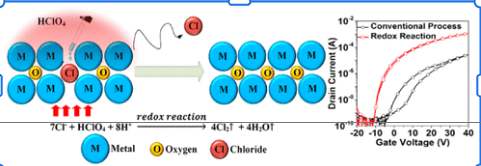
\includegraphics[width=12cm,height=10cm,keepaspectratio]{figures/fig5.png}}
		\caption{The reaction mechanism of the redox reaction(Chen et al)}
		\label{fig:hysteresis}
	\end{figure}
	
	
	
	\section{Applications in energy conversions}
	\subsection{Photo-electro-chemical splitting of water}
	One of the most extensively investigated applications of metal oxide semiconductors is in photo-electro-chemical (PEC) water splitting for sustainable hydrogen production. Hydrogen is a green fuel and more sustainable as compared to the current crude based fuels. Hence it is needed to find a better method to produce Hydrogen without being dependent on hydrocarbon based raw materials such as Methane or coal. The electrochemical decomposition of water is one such method.
	
	The electrosynthesis technique plays a crucial role in developing composite electrocatalyst-semiconductor systems. Examples of such systems are iron oxyhydroxide/nickel oxyhydroxide (FeOOH/NiOOH) deposited on hematite ($Fe_2O_3$) or bismuth vanadate ($BiVO_4$), cobalt oxyhydroxide (CoOOH) on various semiconductor absorbers, and nickel oxyhydroxide (NiOOH) on silicon or III-V semiconductors \cite{Nellist2016}. The presence of MOS and catalyst overlayers substantially improve photo-voltage generation, reaction kinetics, and long-term stability of photo-electrodes by optimizing charge transfer processes at the semiconductor-electrolyte interface and providing catalytically active sites for oxygen evolution reactions. Electrochemically formed oxides provide better hole transfer, reduced Fermi-level pinning and stronger charge accumulation capability. These oxide layers (NiOOH, CoOOH, $MnO_x$) can protect underlying photo-electrode from corrosive electrolytes during the oxygen evolution reaction (OER).
	
	More examples of advancements in this field include the surface electrodeposition of indium oxyhydroxide (InOOH) on titanium-doped $Fe_2O_3$ electrodes, which enhances the PEC oxidation of water \cite{Zhang2019}. Often by having the deposition of another metal oxide layer, the potential drop in the Helmholtz layer can be seen (which was initially absent in Ti-doped $\alpha Fe_2O_3$). \textbf{In electrochemistry, the Helmholtz layer is the compact layer of ions immediately next to the deposition surface.} Using this method we can also spatially direct the growth of MOS particles and hence improving the characteristics of these devices in improving the light absorbing properties.\cite{Rajeshwar2004}
	\begin{figure}
		\centering
		\fbox{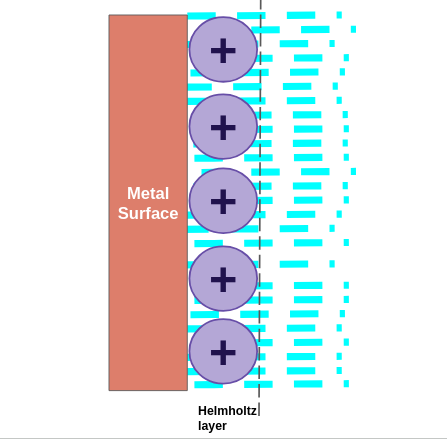
\includegraphics[width=12 cm, height=10 cm]{figures/figd}}
		\caption[Representation of the Helmholtz layer]{In this figure,the circles with the plus charge represent cations. The blue dashed lines represent the solution in which the electrodepostion occurs}
		\label{fig:hysteresis}
	\end{figure}
	
	
	
	Haynes et. Al talk about the templated electrodeposition of cuprous oxide ($Cu_2O$) nanorod arrays. This synthesis represents another significant development in photocatalytic materials \cite{Haynes2015}. The templated electrosynthesis provides a high surface area and directional charge transport pathways, enhancing photocatalytic performance for solar energy conversion and environmental remediation applications. It also gives a more controlled morphology over the MOS device. The templated electrosynthesis of zinc oxide nanorods exemplifies this capability, producing highly ordered one-dimensional nanostructures with excellent electron transport characteristics perpendicular to the substrate. \cite{Lai2006} Here, polycarbonate membranes were used to reduce the temperature from 90 ℃ to 22 ℃..
	
	\subsection{Quantum Dot Sensitized Solar cells}
	Electrosynthesized metal oxide semiconductors such as titanium dioxide ($TiO_2$) and zinc oxide ($ZnO$) serve as critical photo-anode in quantum dot sensitized solar cells (abbreviated as \textbf{QDSSCs}). Quantum dots can be called as artificial atoms and are tiny semiconductor nanocrystals. They are nano-scale semiconductor device structures that exhibit superior optical and electronic properties arising from quantum mechanical effects unique to their extremely small size. The work done by Tian et. Al. has been a major breakthrough and a starting point for development of such structures. \cite{Tian2015}. The control over nanostructure morphology and inter-facial properties can be achieved only through electrochemical synthesis. It also enables optimization of electron injection from photo-excited quantum dots into the metal oxide semiconductor matrix, reduction of inter-facial recombination losses, and enhancement of overall power conversion efficiency. 
	
	\subsection{Photo-voltaic applications} 
	Broader applications in photovoltaic solar energy conversion have been enabled by advances in electrosynthesis of metal oxide semiconductors \cite{Rajeshwar2004}. The integration of electrosynthesized materials in photovoltaic architectures benefits from the precise compositional control and morphological tunability inherent to electrochemical deposition methods, facilitating the development of tandem and multi-junction solar cell configurations with optimized band-gap engineering.
	
	\subsection{Photo-electronic device}
	Metal oxide thin films that can be processed from deposition techniques and material growth techniques have enabled advances in fabrication of electronic and photonic device \cite{Hossein-Babaei2017}. Catalytic metal-accelerated crystallization of metal oxide semiconductors is an innovative approach to enhancing material quality while maintaining low temperatures and costs \cite{Chen2015}. These developments help to facilitate the combination of metal oxide semiconductors in display technologies, light-emitting devices, photo-detectors, and optical modulators. Such interfacial engineering approaches complement the synthesis methods and enable practical implementation of electrosynthesized materials in functional devices. 
	
	\section{Applications in Energy storage}
	\subsection{Super-Capacitor electrodes}
    The continuous electrodeposition of ternary metal oxide nanocomposites represents a very significant advancement in supercapacitor technology, yielding high-efficiency energy storage devices \cite{Ansari12111873}. This synthesis approach enables the fabrication of composite electrode materials with synergistic properties derived from multiple metal oxide components, resulting in an enhanced specific capacitance, improved rate capability, and extended cycling stability. The review by Ansari et. al. emphasizes the promise of electrochemical methods, but it also highlights the necessity for continued improvement to engineer existing metal oxides and composites for high-performance applications.  

	\subsection{Uses as Materials in batteries}
	MOS devices find extensive application as electrode materials in various battery technologies, including lithium-ion, sodium-ion, and multivalent ion batteries. The controlled morphology and composition achievable through electrochemical synthesis enables improvements in ionic and electronic conductivity, accommodation of volume changes during charge-discharge cycling and enhancement of inter-facial charge transfer kinetics. Recent investigations into composite electrode materials of metal oxides for advanced energy storage applications demonstrate the versatility of electrosynthesis in creating hierarchical structures and functional composites \cite{Pazhamalai2024}.
	
	\section{Applications as Sensors}
	
	\subsection{Gas Sensors and Chemiresistive Devices}
	The engineering of MOS nanostructures through electro-synthesis has enabled significant advances in chemiresistive gas sensing, particularly for early warning systems in electrical batteries \cite{PingLi2025}. The controlled synthesis of different nano-sized morphologies, including porous quasi-nanospheres, hollow nanospheres, nanorods, nanosheets, and flower-shaped particles, facilitates optimization of surface-to-volume ratio and active site accessibility, thereby enhancing the selectivity of sensors and response kinetics \cite{Dutta2023}. 
	
	MOS devices with heterojunctions that synthesized through electrochemical methods exhibit superior performance in the detection of volatile organic compounds (VOCs) due to their enhanced hetero-junctionality. Hetero-junctionality is the property which modulates charge carrier depletion regions and improves sensing response characteristics \cite{Zhang2024}. MOS made using electro-chemical methods are attractive for real-time environmental monitoring and industrial process control applications. They have a fast response time and wide range of adjustable sensitivity which makes them desirable.
	\subsection{Biosensors}
	For monitoring enzymatic reactions and foor diagnostic purposes, MOS based biosensors fabricated through electrosynthesis demonstrate exceptional performance characteristics \cite{Dutta2023}. The capability to create enzyme-immobilized nanostructures through these methods facilitates highly sensitive and selective bio-analytical platforms. The high sensitivity, accuracy, and rapid response time of electrosynthesized metal oxide semiconductor biosensors position them as valuable tools in clinical diagnostics, food safety monitoring, and environmental analysis.
	\section{Fuel Cell Technologies}
	Electrosynthesis techniques for thin-film functional layers in solid oxide fuel cell (SOFC) technology present significant opportunities for advanced energy conversion systems \cite{Kalinina2025} The most promising applications of electrolytic deposition methods are anticipated in the fabrication of protective coatings and highly active electrodes for intermediate and low-temperature SOFCs. While challenges remain in creating gas-tight solid electrolyte layers and thick-film electrodes based on the materials and composites through electro-deposition, the current research continues to expand the viability of electrochemical synthesis routes in fuel cell component fabrication.
	\section{Catalytic and Electrocatalytic Applications}
	The electrodeposition of nano- and micro-materials has yielded significant advancements in making cataysts for diverse electrochemical applications \cite{Tovaroliva2024}. Galvanostatic electrodeposition strategies enable precise tuning of functional material structures through controlled manipulation of electrode kinetics, potential drift phenomena, and oscillatory deposition behavior. Such type of synthesis methods facilitate the development of electro-catalysts with an optimized active site distribution, electrical conductivity, and mass transport characteristics for applications including water electrolysis, $CO_2$ reduction, and nitrogen fixation.
	
	\section{Plasmonics and Optoelectronic Applications}
	Hydrogen-doped MOS synthesized through electrochemical methods exhibit exceptional and tunable LSPR phenomena.  The doping of MOS offers an inexpensive alternative to noble metal-based plasmonic materials \cite{Cheng2016}. Cheng et. al. discuss this method of synthesizing hydrogen-doped MOS. The substitution of  noble metals for plasmon resonances allows the LSPR to be obtained at 565 nm i.e. in the visible light range. 

	Visible-light-active doped metal oxide nanoparticles prepared through electrosynthesis find applications in photocatalysis, chemosensing, and photovoltaics \cite{Medhi2020}. The ability to introduce a controlled dopant concentrations through electrochemical methods enables tuning the optical absorption, carrier mobility, and photo-catalytic activity for specific application requirements.
	
	The range of applications of electrosynthesized metal oxide semiconductors continues to broaden as research continues to tackle notable basic science questions and as novel materials systems continue to be researched. Electrochemical methods for the synthesis of rare earth metal oxide semiconductors may provide novel optical and magnetic features necessary for specialized functionality or applications \cite{Patil2022} Theoretical studies and atomistic simulations that have examined the mechanistic aspects of metal electrodeposition provide fundamental studies and information that can be used to optimize experimental studies \cite{Kalinina2025}, and enable rational design of synthesis protocols to generate next-generation materials.
	
	% == Chapter 5 conc ==
	\chapter{Conclusion}
	This review establishes that defect engineering, controlled deposition, and dopant manipulation significantly influence device efficiency and long-term stability. Continued work on hybrid approaches combining perovskites and oxide nanocomposites can accelerate progress in sustainable electronics. 
	
	The electrosynthesis of metal oxide semiconductors has shown exceptional flexibility across a variety of technological applications. As examples, basic electronics such as MOSFETs and memory elements; energy conversion and storage applications including PEC water splitting, solar cells, supercapacitors, and batteries all can use a significant advantage from the electrochemical synthesis route of metal oxide semiconductors, including compositional control, tunable morphology, fabrication at low temperatures and scalable processing. Sensing applications based on the high surface area and tunable electronic properties of electrosynthesized metal oxide semiconductors have achieved substantial commercial success, while even more recent applications in fields such as plasmonics, catalysis, and fuel cells provide new avenues for technological impact of electrosynthesis of metal oxide semiconductors.
	As electrosynthesis techniques continue to progress through a deepening fundamental understanding of electrochemical mechanisms and interfacial phenomena in metal oxide semiconductors, even more potential for innovation across metal oxide semiconductor technologies will be realized. For example, integrating machine learning approaches to optimize electrodeposition processing; developing in-situ characterization techniques for real-time monitoring of electrodeposition; developing new electrolyte formulations and applied potential profiles are examples of highly promising and exciting directions for future work. Furthermore, as the demand for sustainable and economically viable energy efficient synthesis techniques continues to grow, the process of electrosynthesis of metal oxide semiconductors will become a more important approach to sintering and fabricating functional materials for an even wider range of applications.
	% === REFERENCES ===
	\addcontentsline{toc}{chapter}{References}
	\bibliographystyle{apacite}
	\bibliography{references}


	
	
	% === NOMENCLATURE (if needed) ===

\end{document}


